\chapter{Application to Markov chain Monte Carlo algorithms}
\label{ch:mcmc}
One of the interesting applications of $\gradTD$ learning is in the context of Markov chain Monte Carlo (MCMC) simulations. In this chapter, a basic introduction to MCMC algorithms with a particular emphasis on Langevin diffusion and its discrete variants is provided first in \Section{s:mcmc_langevin}. We then define asymptotic variance as a measure of convergence and motivate how $\gradTD$ learning is perfectly suited to obtain MCMC estimates with minimal asymptotic variance. In \Section{s:mcmc_metropolis}, we describe the very popular Metropolis-Hastings (MH) algorithm and present an extension of the asymptotic variance reduction methods to the class of reversible Markov chains in \Section{s:mcmc_reversible_mc_cv}. A majority of the existing research that aims to improve the convergence of MCMC estimates focuses on minimizing the variance. Although, this is easier to implement, in \Section{s:mcmc_var_vs_asym_var}, through a motivating example, we illustrate why this is not the correct objective for MCMC. 
In recent research, it has been found that under certain assumptions, the asymptotic variances of certain well-known MCMC algorithms such as the Unadjusted Langevin Algorithm (ULA) and Random Walk Metropolis (RWM) are close (upto a scaling factor) to the asymptotic variance of the Langevin diffusion \cite{brodurmeymourad18}. Hence, the application of the same control variate techniques is justified.  Applications to numerical examples in one-dimension and a logistic regression (logit) is discussed in \Section{s:mcmc_numerics}. 
 % \anandspm{sample variance or ordinary variance, what is the right term?} 
 %\anand{Need to rephrase after reading \cite{brodurmeymourad18}}
\section{Langevin Diffusion for MCMC}
\label{s:mcmc_langevin}
In many scenarios, it is of interest to compute the expectation of a function $c$ with respect to a target distribution $\pr$:
\begin{equation}
\eta = \int c(x)\pr(x)\ud x\, .
\label{e:eta}
\end{equation} 
Typically, computing integrals of the form \eqref{e:eta} analytically is difficult when $\pr$ is in high dimensions. Markov chain Monte Carlo (MCMC) provides numerical algorithms to obtain estimates of $\eta$. It can be approximated using time averages of the following form:
\begin{equation}
\eta_N =\frac{1}{N}\sum_{n=0}^{N-1} c(\markovstate_n),
\label{e:sample_mean_HM}
\end{equation}
in which $\boldsymbol{\markovstate}$ is a Markov chain whose steady-state distribution has density $\pr$ \cite{asmgly07,MT}.
In this chapter, we initially focus on a formulation in continuous time and then extend the idea to discrete-time MCMC algorithms.

The Langevin Diffusion, introduced in \Section{s:langevin_diffusion} is the grandmother of all MCMC algorithms. It forms the basis for other MCMC algorithms such as the Unadjusted Langevin algorithm (ULA) and Metropolis-adjusted Langevin algorithm (MALA). The diffusion obeys the SDE in \eqref{e:diff_td_langevin_cts}:
\begin{equation}
\ud \markovstate_t = - \nabla \pot(\markovstate_t) \, \ud t+  \sqrt{2} \, \ud W_t,
\label{e:mcmc_langevin_cts}
\end{equation}
where $\bfmW=\{W_t : t\ge 0\}$ is a standard Brownian motion on $\Re^d$.
Under general conditions, this diffusion is reversible, with unique invariant density $\pr=e^{-U +\Lambda}$,  where $\Lambda$ is a normalizing constant so that $\pr$ integrates to unity.  For a large $T$, the mean $\eta$ can be approximated as,
\begin{equation}
\eta \approx \eta_T \eqdef \frac{1}{T}\int_0^T c(\markovstate_t) \, dt.
\label{e:mcmc_lang_mean_cts}
\end{equation}

To compare the different MCMC algorithms it  is convenient to consider an asymptotic setting.   Under general conditions, the estimates will obey a Central Limit Theorem (CLT) of the form:
\begin{equation}
\sqrt{T} \tileta_T \xrightarrow[]{d} N(0,\asymvar)
\end{equation}
where $\tileta_T =\eta_T-\eta$, and the convergence is in distribution.   Under further mild assumptions,  the variance of the Gaussian limit is given by the so-called asymptotic variance:
\begin{equation}
\asymvar = \lim_{T \to \infty} \Expect \left[\left(\frac{1}{\sqrt{T}}\int_{0}^{T}(c(\markovstate_t)-\eta)dt\right)^2\right]
\label{e:aVar}
\end{equation}
For example, these conclusions hold for a Markov chain that is $V$-uniformly ergodic,  provided $c^2\in\LV$  \cite{glymey96a,MT}. %\anand{$c^2$ or $c$?}
It has been shown in \cite{glymey96a,MT} that the asymptotic variance $\asymvar$ has the following general representation in terms of the solution to Poisson's equation $h$ \eqref{e:diff_td_poissons},
\begin{equation}
\asymvar  =2\langle h, \tilc\rangle_{L^2},
\label{e:avarFish}
\end{equation}
where $\tilc \eqdef c - \eta$. 
The representation \eqref{e:avarFish} is valid for any diffusion that is $V$-uniformly ergodic.
For the special case of the Langevin diffusion,  by application of \Prop{prop:lang_generator_grad}, $\asymvar = 2 \| \nabla h \|^2_{L^2}$.

In practice, discretized versions of the equation based on Euler-Mauryama scheme are used \eqref{e:diff_td_langevin_discrete}:
\begin{equation*}
\markovstate_n = \markovstate_{n-1} - \nabla U(\markovstate_{n-1}) \mcmcstep_{n} + \sqrt{2  \mcmcstep_{n-1}} W_{n-1} ,
\end{equation*}
where $\{\mcmcstep_n\}_{n\geq 1}$ is a sequence of step sizes and $\{W_n\}_{n\geq 1}$ is a sequence of i.i.d. standard Gaussian random variables. This implementation is called the Unadjusted Langevin algorithm (ULA) and was introduced as a means to sample from a target density $\pr$ in the physics literature by \cite{par81}. In the numerical experiments that follow, the step size $\mcmcstep$ is chosen to be a constant, independent of $n$. 

The primary goal in the design of MCMC algorithms is the faster convergence of the Markov chain to its invariant distribution (i.e. the target distribution). The asymptotic variance is a measure of this convergence and hence, it is ideal to minimize $\asymvar$. Several approaches have been proposed to improve the convergence rate including constructing an irreversible Markov chain with the same invariant density \cite{hwanorwu15, dunlelpav16}, using an optimal scaling parameter \cite{robros01} etc. Most of these approaches alter the transition kernel of the Markov chain and hence, do not work well on samples already obtained. In the remainder of this paper, we restrict our discussion to post-hoc schemes for reversible Markov chains, i.e. samples from an ergodic Markov chain are available and variance reduction is achieved by post-processing. These schemes require no changes to the sampling methodology. 

Control variates introduced in \cite{HenThesis,henmeytad03a,kimhen07,ctcn} are zero-mean terms, which when added to the estimator can produce a significant reduction in the asymptotic variance without adding bias. One of the advantages of this scheme is that they work post-hoc, and are independent of the MCMC algorithm used. %\anand{a few more words on original application}

Dellaportas et al. in \cite{delkon12} have employed control variates for particular examples of reversible Markov chains like the Gibbs sampler.
More recently, Brosse et al. in \cite{brodurmeymou18} show that the asymptotic variances of ULA, MALA and RWM are close to the asymptotic variance of the Langevin diffusion and construct Langevin-based control variates that work for all the three methods. In this dissertation, we borrow heavily from both the above and demonstrate that using RKHS based $\gradTD$ learning algorithms, the variance reduction is improved many-fold. 

The basic idea is described here. Let $\psi\colon\Re^d\to\Re^\ell$ denote a $C^2$ function, regarded as a family of $\ell$ basis functions, and $\param\in\Re^\ell$ denote the parameters,
\begin{equation}
\begin{aligned}
c^\param  \eqdef c + \underbrace{\generate h^\param}_{\text{Control variate}},
\qquad
\text{where}
\quad
h^\param  \eqdef  \sum_{i=1}^\ell \param_i \psi_i = \param^\transpose \psi\,
\end{aligned}
\label{e:mcmc_h_and_c}
\end{equation}
and $\generate$ denotes the differential generator of the Langevin diffusion \eqref{e:diff_td_langevin_generator}. 
Under the assumptions imposed it will follow that the steady-state means of $c$ and $c^\param$ coincide for any $\param\in\Re^\ell$,  so that we obtain a family of asymptotically unbiased estimators: % \anand{Do we need to show $Ph = h$?}
\begin{equation}
\eta^\param_T =\frac{1}{T}\int_0^T c^\param(\markovstate_t)  \, dt
\label{e:mcmc_eta_theta}
\end{equation}
It is then of interest to find the parameter with minimal asymptotic variance:
\begin{equation}
\param^* = \argmin_\param {\asymvar}_{,\param}
\label{e:mcmc_theta_star}
\end{equation} 
Here, ${\asymvar}_{,\param}$ corresponds to the asymptotic variance of the new estimate \eqref{e:mcmc_eta_theta}, i.e.
\[
\sqrt{T} (\eta^\param_T - \eta ) \xrightarrow[]{d} \mathcal{N} (0,{\asymvar}_{,\param}).
\]

\begin{proposition}
	\label{t:mcmc_say_var_cv}
	Suppose that  $c$ and each $\psi_i$ lie in $\LsqrV$. Then, equation \eqref{e:mcmc_eta_theta} defines an asymptotically unbiased estimate of $\eta$. Its asymptotic variance is
	\begin{equation}
	{\asymvar}_{,\param}
	= 2  \| \nabla  h - \nabla h^\param  \|^2_{L^2}
	\label{e:mcmc_asy_var_cv}
	\end{equation}
\end{proposition}

\begin{proof}
	Applying the differential generator $\generate$ on $h - h^\param$, we have
	\begin{equation}
	\begin{aligned}
	\generate ( h -h^\param) & = - \tilc - \generate h^\param\\
	& = - c + \eta + c - c^\param  \qquad \text{From \eqref{e:mcmc_h_and_c}} \\
	& = - c^\param + \eta\, \eqdef -\tilc^\param
	\end{aligned}	
	\label{e:mcmc_proof_i}
	\end{equation}
	Hence $h-h^\param$ is the solution to Poisson's equation with forcing function $c^\param$. Analogous to \eqref{e:avarFish}, the asymptotic variance for the new estimator in \eqref{e:mcmc_eta_theta} is represented as ${\asymvar}_{,\param} = 2 \langle h - h^\param, \tilc^\param \rangle_{L^2}$, and applying \Prop{prop:lang_generator_grad} gives \eqref{e:mcmc_asy_var_cv}.
\end{proof}

An important observtion here is that the asymptotic variance ${\asymvar}_{,\param}$ for the new estimator \eqref{e:mcmc_h_and_c}, with control variates \eqref{e:mcmc_asy_var_cv} has the same form as the norm in \eqref{e:diff_td_gradTD_norm_error}, and hence any of the variants of the $\gradTD$ algorithm can be applied can be applied to minimize it. Numerical examples using these algorithms are discussed in \Section{s:mcmc_numerics}.

\section{Metropolis-Hastings Algorithm}
\label{s:mcmc_metropolis}
Although Langevin diffusion offers a very intuitive sampling algorithm, it requires the computation of the gradient of the potential function $U$, which may be expensive in high dimensions. Hence, other discrete time algorithms are preferred. Metropolis-Hastings algorithm is a popular MCMC technique to simulate multivariate distributions. It was originally proposed by Metropolis in 1953 and extended to a more general case by Hastings in 1970 \cite{has70}. The only requirement in Metropolis-Hastings is that it should be possible to compute the value of a function $f$ proportional to the target density $\pr$. The function $f$ could potentially be the unnormalized form of $\pr$.

The algorithm requires the choice of a simple ``proposal'' distribution $g$, from which samples can be drawn easily. The function $g(x,y)$ gives the conditional distribution for the next sample $y$, given the current sample $x$.  The algorithm can be summarized in the following steps:

\begin{algorithm}{Metropolis-Hastings Algorithm}
	\begin{algorithmic}[1]
	\Require $f(x) \propto \pr(x), g(x,y)$
	\Ensure Samples $\{\markovstate_i\}_1^N \sim \pr$
	\State Choose an arbitrary point $\markovstate_0 = x$ to be the first sample.
	\State Pick a new candidate sample point $x' \sim g (x,.) $ according to the proposal distribution.
	\State Compute the acceptance ratio $\alpha(x,x')= \min \left[ \frac{f(x') \, g (x',x)}{f(x) \, g(x,x')}, 1\right] $.
	\State With probability $\alpha$, accept $x'$ and set $\markovstate_1 = x'$; if rejected set $\markovstate_1 = x$.
	\State Repeat above for $ \markovstate_2, \hdots \markovstate_N$ for a fixed $N$.
	\end{algorithmic}
\end{algorithm}
% If $g$ is chosen to be Gaussian, due to symmetry $g(x,y) = g(y,x)$. This simplifies the computation of the acceptance ratio $\alpha$.

The transition kernel $P_{mh}$ for a Metropolis-Hastings chain can be written as:
\begin{equation}
P_{mh}(x,dy) \eqdef g(x,y) \alpha(x,y) dy + \left [ 1 - \int_{\state} g(x,y) \alpha(x,y) dy \right] \delta_x (dy),
\label{e:kernel_mh}
\end{equation}
and with the acceptance ratio $\alpha$ as defined, the reversible Markov chain with kernel $P_{mh}$ has its invariant density as $\rho$.

A special case of this algorithm is obtained if $g$ is chosen to be a Gaussian centered at $x$ with $\mcmcstep$ as the variance parameter. This also simplifies the expression for $\alpha$ as $g(x,x') = g(x',x)$. This variant is known as the random walk Metropolis (RWM) algorithm. For a small value of $\mcmcstep$, it has been shown by Brosse et al. in \cite{brodurmeymourad18} that the following relation between $P_{mh}$ and the differential generator $\generate$ of the Langevin diffusion holds, %\anand{variance parameter is equivalent to the time step in ULA?}
\[
\lim_{\mcmcstep \to 0^+} \mcmcstep^{-1} (P_{mh} - I) = \generate
\]
Thus for small values of $\mcmcstep$, the control variates can be obtained as $\mcmcstep \generate h^\theta$. %\rd{But this approximation is not valid for larger step-sizes and hence this method is practically limited in use.} %\anand{Do we need this statement? Or is there a hack for larger $\mcmcstep$? }

\section{Control Variates for a Reversible Markov Chain} 
\label{s:mcmc_reversible_mc_cv}
In this section, we extend the idea of control variates to the more general case of reversible Markov chains, including RWM. The main difficulty is that \Prop{prop:lang_generator_grad} is absent here. However using reversibility, we obtain an expression for the optimal parameter values. A derivation similar to this is presented in \cite{delkon12}.
Consider a discrete time Markov chain with a transition kernel $P$.  Let $h$ denote the solution to the Poisson's equation of this Markov chain,
\[
(P - I) h = -\tilc,
\]
where $I$ refers to the identity operator.
In discrete time, the asymptotic variance has the following representation in terms of $h$,
\begin{equation}
\asymvar = 2 \langle h, \tilc \rangle_{L^2} - \langle \tilc, \tilc \rangle_{L^2}.
\label{e:mcmc_avar_reversible}
\end{equation}
A linearly parameterized class of functions $h^\param$ is defined as in \eqref{e:mcmc_h_and_c} and a new function $c^\param$ with the control variates is defined as
\begin{equation}
c^\param \eqdef c +  (P - I) h^\param
\label{e:mcmc_discrete_cv}
\end{equation}
Denoting $\tilh^\param \eqdef h - h^\param$, a simple extension of \eqref{e:mcmc_proof_i} is obtained:
\begin{equation}
(P - I) \tilh^\param = -\tilc^\param.
\label{e:mcmc_discrete_poissons_cv}
\end{equation}
Following \eqref{e:mcmc_avar_reversible}, the asymptotic variance corresponding to this new estimator $c^\param$ has the following representation:
\begin{equation}
\begin{aligned}
{\asymvar}_{,\param} \eqdef & 2 \langle \tilh^\param, \tilc^\param \rangle_{L^2} - \langle \tilc^\param, \tilc^\param \rangle_{L^2}\\
= &  - 2 \langle \tilh^\param, (P - I) \tilh^\param \rangle_{L^2} -\langle (P - I) \tilh^\param, (P - I) \tilh^\param \rangle_{L^2}\\
= & \langle \tilh^\param, \tilh^\param \rangle_{L^2} - \langle P \tilh^\param, P \tilh^\param \rangle_{L^2}
\label{e:mcmc_asym_var_theta_discrete}
\end{aligned}
\end{equation}
To eliminate the unknown term $h$ from \eqref{e:mcmc_asym_var_theta_discrete}, the self-adjoint property of the transition kernel of a reversible Markov chain is used (\Prop{theorem:self_adjoint}).
\begin{proposition}
	\label{theorem:self_adjoint}
	For a reversible Markov chain the following holds:
	\[
	\langle P f , g \rangle_{L^2}= \langle f, P g \rangle_{L^2}, \qquad f,g \in L^2(\pr)
	\]
\end{proposition}
\begin{proof}
	For a reversible Markov chain, the detailed balance equations hold with respect to its unique invariant measure $\pr$:
	\begin{equation}
	\pr(dx) P(x,dy ) = \pr(dy) P(y,dx).
	\label{e:det_bal}
	\end{equation}
	From the definition of the transition kernel $P$,
	\begin{equation}
	\begin{aligned}
	P f (x) & = \Expect [f(\markovstate_{k+1}) | \markovstate_k = x] \\
	& = \int P(x,dy) f(y)
	\label{e:trans_kernel}
	\end{aligned}
	\end{equation}
	Using the definition of the inner product,
	\[
	\begin{aligned}
	\langle P f, g \rangle_{L^2} & \eqdef \int (Pf(x)) g(x) \pr(dx) \\
	& = \int \left(\int P(x,dy)f(y)\right) g(x) \pr(dx)  \qquad (\text{From } \eqref{e:trans_kernel}) \\
	& = \int \left(\int P(y,dx) g(x) \right) f(y) \pr(dy) \qquad (\text {Applying } \eqref{e:det_bal})\\
	& = \int (P g(y)) f(y) \pr(dy) \\
	& = \langle f, P g \rangle_{L^2}.
	\end{aligned}
	\]
\end{proof}

\begin{proposition}
	\label{t:theta_discrete}
	The optimal parameter vector $\param^* \in \Re^\ell$ that minimizes \eqref{e:gamma_discrete} is given by
	\begin{equation}
	\begin{aligned}
	\param^* & \eqdef M^{-1} b \qquad \text{where,} \\
	M &\eqdef \langle \psi, \psi \rangle_{L^2}- \langle P \psi,  P \psi \rangle_{L^2} \\
	b & \eqdef  \langle \tilc, \psi \rangle_{L^2} +  \langle \tilc, P \psi \rangle_{L^2}.
	\end{aligned}
	\label{e:theta_star_discrete}
	\end{equation}
	The optimal control variate is then given by,
	\[
	(P-I) h^\param = \param^{* \transpose} (P \psi) - \param^{* \transpose} \psi.
	\]
\end{proposition}
\begin{proof}
	Expanding the expression for ${\asymvar}_{,\param}$ \eqref{e:mcmc_asym_var_theta_discrete} gives,
	\begin{equation}
	\begin{aligned}
	{\asymvar}_{,\param} & = \langle \tilh^\param, \tilh^\param \rangle_{L^2} - \langle P \tilh^\param, P \tilh^\param \rangle_{L^2} \\
	& = \langle h, h \rangle_{L^2} - 2 \langle h, h^\param \rangle_{L^2} + \langle h^\param , h^\param \rangle_{L^2} - \langle P h, P h \rangle_{L^2} + 2 \langle P h , P h^\param \rangle_{L^2} - \langle P h ^\param , P h^\param \rangle_{L^2}
	\label{e:gamma_discrete}
	\end{aligned}
	\end{equation}
	Substituting for $h^\param$ in \eqref{e:mcmc_asym_var_theta_discrete} and applying the first order necessary conditions for optimality by taking the derivative with respect to $\param$,
	\begin{equation}
	\begin{aligned}
	0 & = - \langle h, \psi \rangle_{L^2} +  \param^{*\transpose} \langle \psi, \psi \rangle_{L^2}+ \langle P h, P \psi \rangle_{L^2}-\param^{*\transpose}  \langle P \psi, P  \psi \rangle_{L^2}  \\
	& = - \langle h, \psi \rangle_{L^2} +  \param^{*\transpose} \langle \psi, \psi \rangle_{L^2}+ \langle P h, P \psi \rangle_{L^2}-\param^{*\transpose}  \langle P \psi, P  \psi \rangle_{L^2}  + \langle P h, \psi \rangle_{L^2} - \langle P h, \psi \rangle_{L^2} \\
	& = - \langle \tilc , \psi \rangle_{L^2} + \langle P h, (P - I) \psi \rangle_{L^2} + \param^{*\transpose} \Bigl( \langle \psi, \psi \rangle_{L^2}  - \langle P \psi, P \psi \rangle_{L^2} \Bigr) \qquad \text{(Using $(P-I) h = -\tilc$)}
	\label{e:mcmc_gradient_reversible}
	\end{aligned}
	\end{equation}
	Applying \Prop{theorem:self_adjoint},
	\[
	\langle P h , (P -I) \psi \rangle_{L^2} = \langle (P - I) h, P \psi\rangle_{L^2} = - \langle \tilc, P \psi \rangle_{L^2}
	\]
	Denoting $M$ and $b$ as
	\[
	M \eqdef \langle \psi, \psi \rangle_{L^2} - \langle P \psi, P \psi \rangle_{L^2}, \qquad b \eqdef \langle \tilc, \psi \rangle_{L^2} + \langle \tilc, P \psi \rangle_{L^2}.
	\]
	completes the proof.
\end{proof}
It can be shown that $M$ is a symmetric positive definite matrix. The Monte Carlo estimates of $M$ are designed to respect this constraint:
\[
\begin{aligned}
\hat{M}_N & \eqdef \frac{1}{N} \sum_{n=0}^{N-1} \Bigl(\psi(\markovstate_n) \cdot\psi^\transpose(\markovstate_n) - \psi(\markovstate_{n+1})\cdot \psi^\transpose(\markovstate_{n+1}) \Bigr) \\
M_N  & \eqdef \frac{1}{2} (\hat{M}_N + \hat{M}_N^\transpose )\\
b_N & \eqdef  \frac{1}{N} \sum_{n=0}^{N-1} \tilc(\markovstate_n)\, \Bigl( \psi(\markovstate_n) + \psi(\markovstate_{n+1}) \Bigr).
\end{aligned}
\]

Similar results for optimal control variates for reversible Markov chains have been obtained in \cite{delkon12}. Although optimal parameter weight estimates $\param_N = M_N^{-1} b_N$ are easy to obtain, the main difficulty is to compute the term $P\psi$ which is part of the control variate defined in \Prop{t:theta_discrete}. In \cite{delkon12}, numerical examples are presented for a class of conjugate random-scan Gibbs samplers for which $P\psi$ is explicitly computable in closed form. 

In this dissertation, we substitute for $(P-I)\basis$ with $\mcmcstep \generate \basis$, which is easy to compute. In \cite{brodurmeymourad18}, it has been shown that in addition to standard conditions for geometric ergodicity of the discretized Markov chain, if the following assumptions are satisfied, as $\mcmcstep \to 0^+$,
\begin{align}
\mcmcstep {\asymvar}_{,\mcmcstep} (c^\param) &= \asymvar(c^\param) + o(1), \\ 
\int c^\param(x) \pr_\mcmcstep(x) dx & = \int c^\param(x) \pr(x) dx + O(\mcmcstep), 
\end{align}
then the substitution is reasonable. Here $\pr_\mcmcstep$ denotes the invariant distribution of the discrete Markov chain. It has been verified that these assumptions are satisfied for ULA, RWM and MALA algorithms under appropriate technical conditions.This justifies the use of Langevin-based control variates for small values of $\mcmcstep$. 

\section{Sample Variance v Asymptotic Variance}
\label{s:mcmc_var_vs_asym_var}
The basic idea behind using control variates to minimize asymptotic variance of the MCMC estimates was discussed in \Section{s:mcmc_langevin}. It requires approximating the value function $h$, which is non-trivial in most cases. A large body of prior research \cite{mirsolimp13, oatgircho,papmirgir14} attempts to achieve better estimates by solving an easier problem. In \cite{papmirgir14}, a parameterized family of control variates is considered as in this dissertation. However, the optimal parameter is chosen to minimize the variance rather than the asymptotic variance. This is well-motivated only  if the samples are i.i.d. 
The unbiased estimator in \cite{papmirgir14} is based on a function $c^{\vartheta}$ of the same form as \eqref{e:mcmc_h_and_c}:
\[
\begin{aligned}
c^\vartheta  \eqdef c + \generate h^\vartheta,
\qquad
\text{where}
\quad
h^\vartheta  =  \sum_{i=1}^\ell \vartheta_i \psi_i = \vartheta^\transpose \psi.\,
\end{aligned}
\]
%Examples include the paper by Oates et al. \cite{oatgircho}, where the problem considered is the minimization of variance by using a new estimator  chosen from within Reproducible kernel Hilbert space (RKHS), and the paper by Mira et al \cite{papmirgir14}, which is similar to the present work.
The quantity minimized is the variance, i.e. $\sigma^2_{\vartheta} = \Expect[(\tilc^\vartheta)^2] = \langle \tilc^\vartheta, \tilc^\vartheta \rangle_{L^2}$, where $\tilc^\vartheta = c^\vartheta - \eta$ resulting in
\begin{equation}
\vartheta^*= \argmin_{\vartheta \in \Re^\ell} \sigma^2_\vartheta  = M^{-1} b
\label{e:mcmc_var_theta_star}
\end{equation}
where $M = \langle \generate \psi,  \generate \psi \rangle_{L^2}$ and $b = - \langle \tilc, \generate \psi \rangle_{L^2}$. This is termed the zero-variance (ZV) algorithm in \cite{papmirgir14}. An interesting observation is that the variance minimization algorithm is equivalent to minimizing the Bellman error technique presented in \eqref{e:fpf_nl_be}.

The important question to be addressed is: does minimizing the variance minimize (perhaps approximately) minimize the asymptotic variance? Using a simple numerical example, it can be shown that this is not always the case.

Consider $\state \equiv \Re$, $c(x) \equiv x $, $\pr$ is a univariate 2-component Gaussian mixture density defined in \eqref{e:fpf_gaussian_mixture_example} and shown by the shaded region in \Fig{fig:mcmc_cv_theta_var}. Two sets of basis functions are chosen for $\psi$ (similar to those defined in \Section{s:linear_param}):
\begin{romannum}
	\item  a family of polynomials of the form $\basis_n(x) = x^n$ for $1 \leq n \leq \ell$.
	\item a family of polynomial functions weighted by the Gaussian density components $\pr_i$,
	\begin{equation}
	\{\psi_n(x) : x\in\Re,\ 1\le n\le \ell\}  = \{ x^k \pr_i(x) :  1\le k \le \ell/2,   \ i=1,2\},
	\label{e:basis}
	\end{equation}
	where $\pr_i \sim N(\mu_i, \sigma^2_i)$. The rationale behind this choice of basis functions is that the contribution of each $\psi_n$ is local to a particular mode.  This allows us to approximate $h$ with good accuracy in the region around $\mu_1$ and $\mu_2$, where most of the samples of the Langevin diffusion are concentrated. 
\end{romannum}

\begin{figure}[htbp]
	\centering
	\mbox{
	\subfigure[]{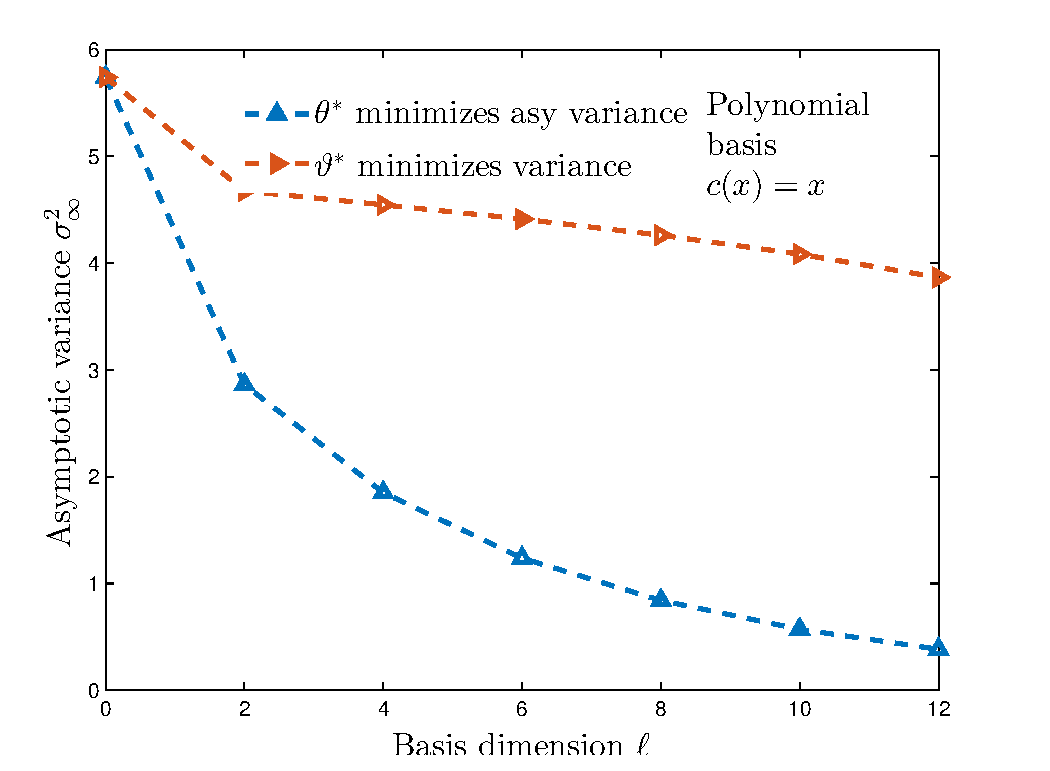
\includegraphics[width=3in]{images/Chap5_x_var_vs_asym_var_poly}} \quad
	\subfigure[]{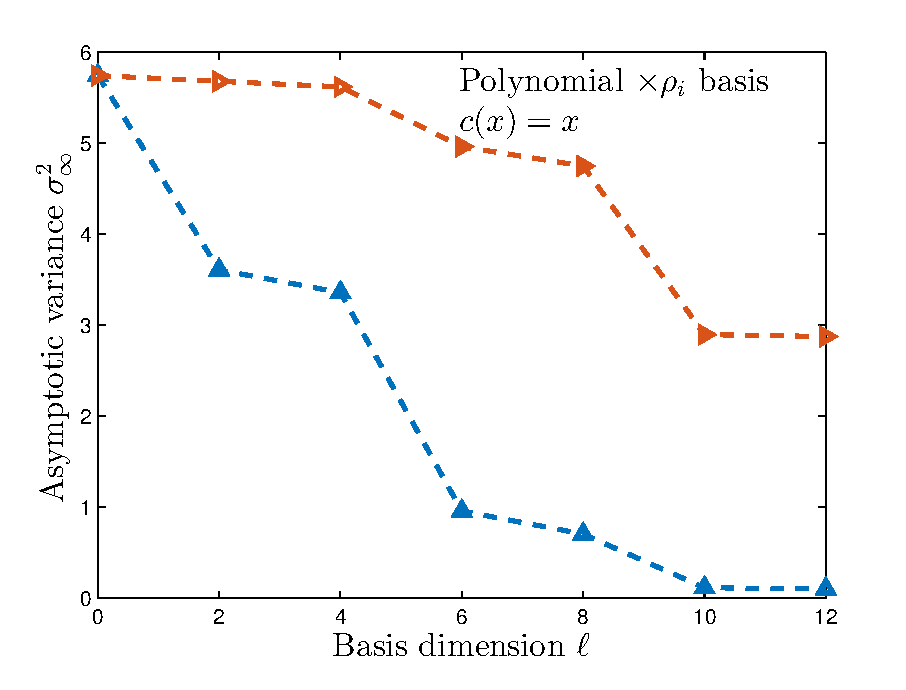
\includegraphics[width=3in]{images/Chap5_x_var_vs_asym_var_wt_poly}}
	% \subfigure[]{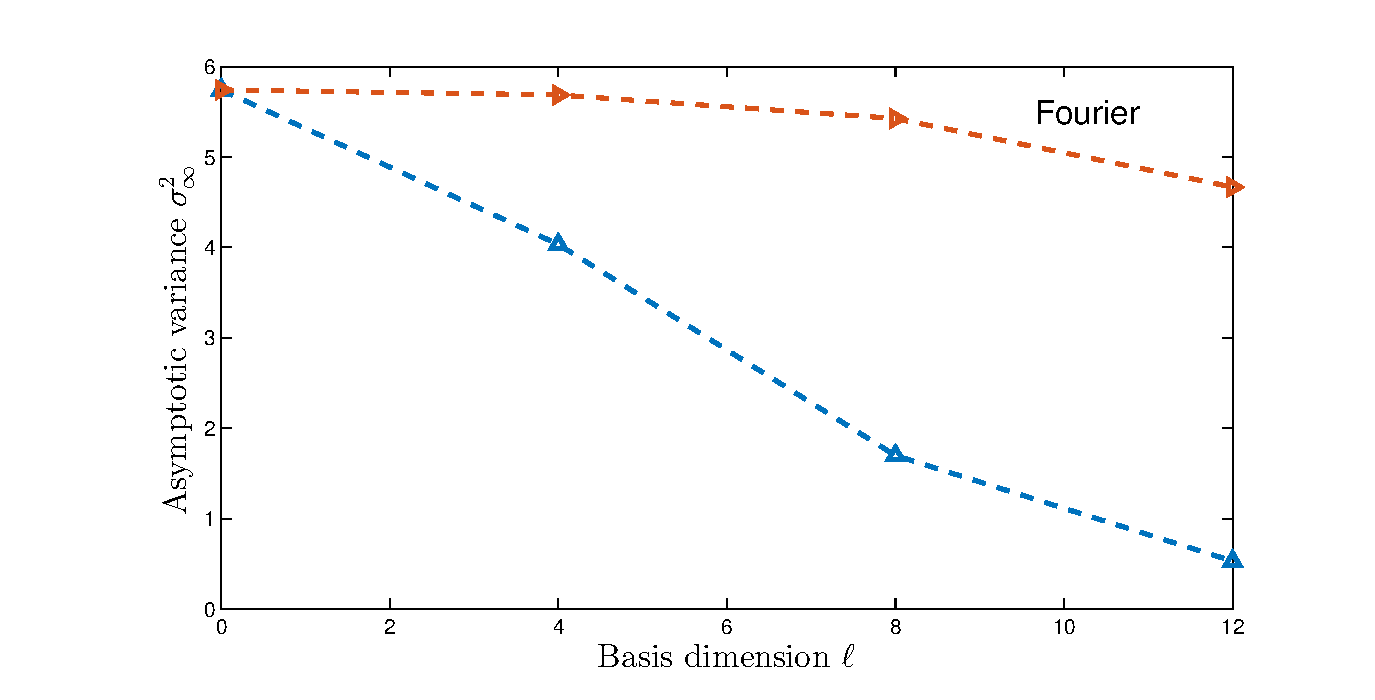
\includegraphics[width=3in]{images/Chap5_x_var_vs_asym_var_fourier}} 
	}

	\mbox{
	\subfigure[]{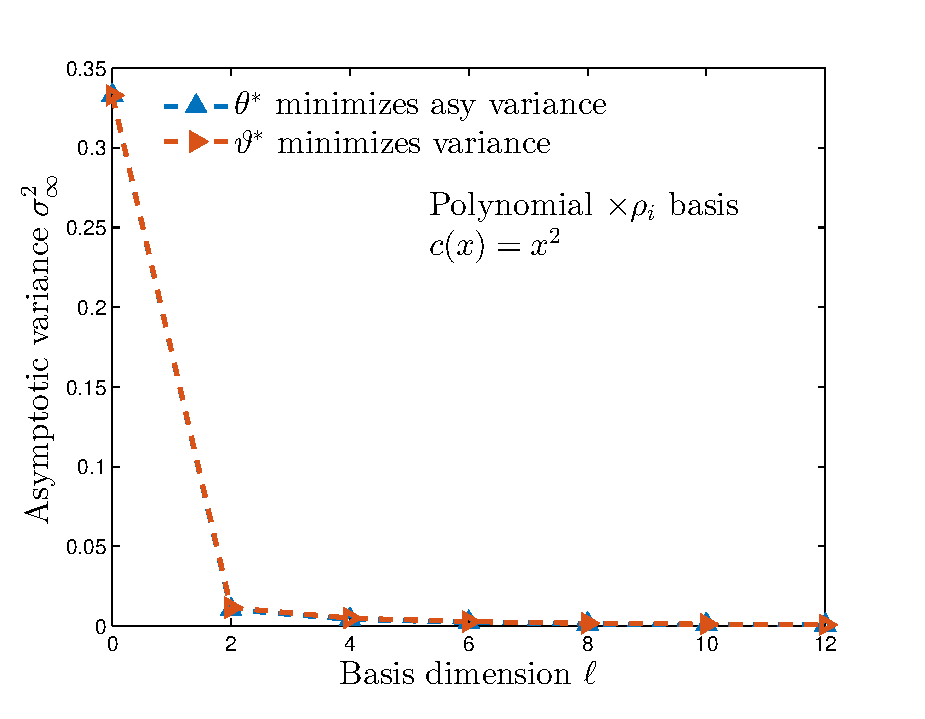
\includegraphics[width=3in]{images/Chap5_x2_var_vs_asym_var_poly}} \quad 
	\subfigure[]{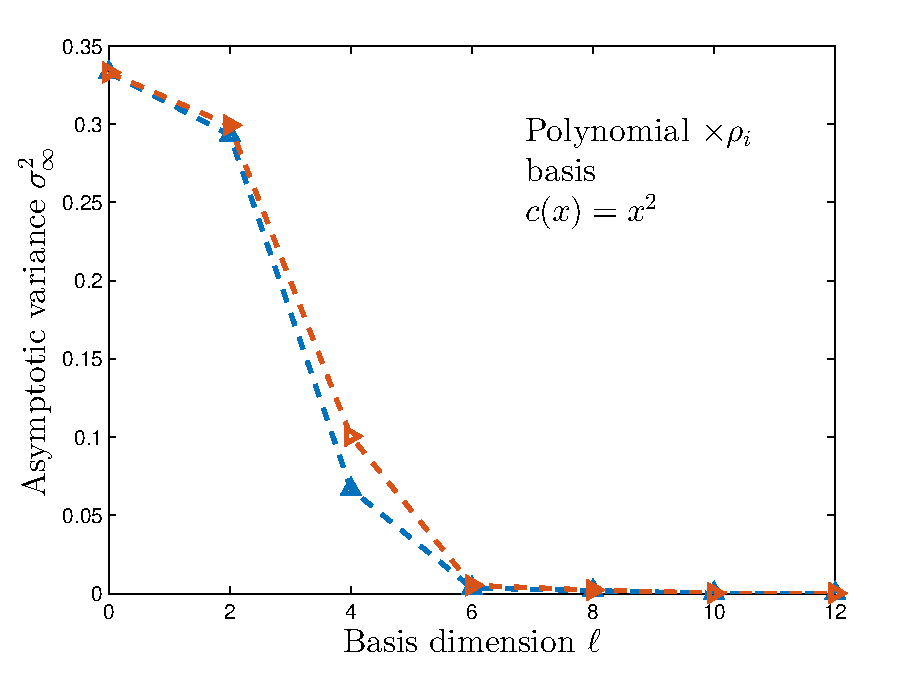
\includegraphics[width=3in]{images/Chap5_x2_var_vs_asym_var_wt_poly}}
	% \subfigure[]{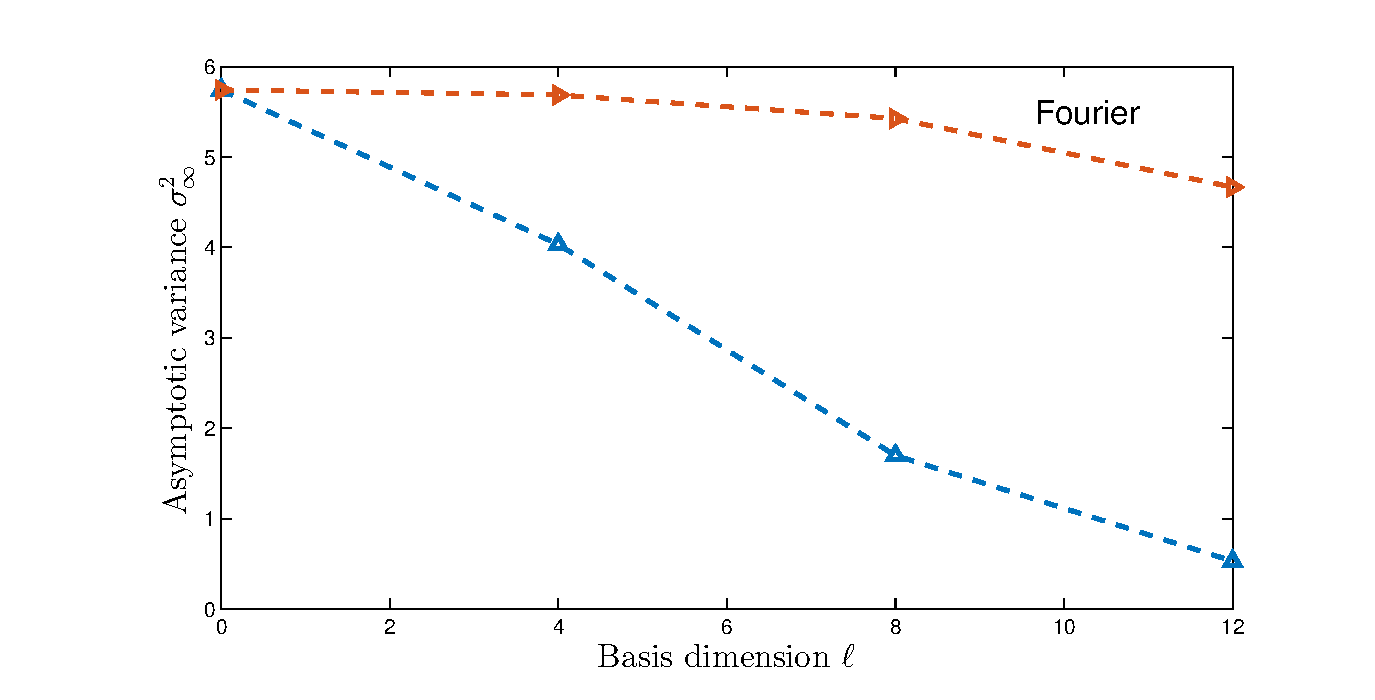
\includegraphics[width=3in]{images/Chap5_x_var_vs_asym_var_fourier}} 
	}
	\caption{Comparison of ${\asymvar}_{,\theta^*}$ and ${\asymvar}_{,\vartheta^*}$ for $\theta^*, \vartheta^* \in \Re^{\ell}$, $0 \leq \ell \leq 12$ and $c(x) = x, x^2$, for i) a polynomial basis (in A and C) and ii) a weighted polynomial basis (in B and D)}
	\label{fig:mcmc_var_vs_asym_var}
\end{figure}

The resulting asymptotic variances for the parameters, $\theta^*$ \eqref{e:mcmc_theta_star} and $\vartheta^*$ \eqref{e:mcmc_var_theta_star} are compared against the basis dimension $\ell$.  The optimality gap for $c(x) = x$, shown in parts A and B of \Fig{fig:mcmc_var_vs_asym_var} is considerable.
The discrepancy is clear from a close look at the two functions $c^{\theta^*}$ and $c^{\vartheta^*}$ that are plotted in \Fig{fig:mcmc_cv_theta_var}. The key difference is that the ``local mean'' of $c^{\theta^*}$ is nearly $\eta$ in each well of the density $\pr$ (shaded region of \Fig{fig:mcmc_cv_theta_var}):
\[
\begin{aligned}
\int_{-\infty}^0 c^{\theta^*}(x) \pr(x)\, dx	
\approx
\int_0^\infty c^{\theta^*}(x) \pr(x) \, dx \approx \eta =0.
\end{aligned}
\]
This helps reduce the asymptotic variance for this slowly mixing diffusion. The function $c^{\vartheta^*}$  does not share this property and produces biased estimates of $\eta$ in each well.
The approximations ${h^{\vartheta^*}}'$ and ${h^{\theta^*}}'$ are plotted along with the exact solution $h'$ obtained analytically in
\Fig{fig:mcmc_cv_theta_var}.  The function ${h^{\vartheta^*}}'$ is a poor approximation to $h'$,  and that results in much higher asymptotic variance. In summary, to minimize the asymptotic variance, it is  important to approximate $h'$ quite well and the $\gradTD$ objective function aims to minimize the approximation error in the mean-square sense. The same experiment was repeated for $c(x) \equiv\sin x$ with similar results. It is conjectured that this phenomenon is more pronounced in multimodal densities. However, for $c(x) = x^2$, both the methods achieve nearly similar reduction in asymptotic variance. 

\begin{figure}[htbp]
	\centering
	\mbox{
		\subfigure []	{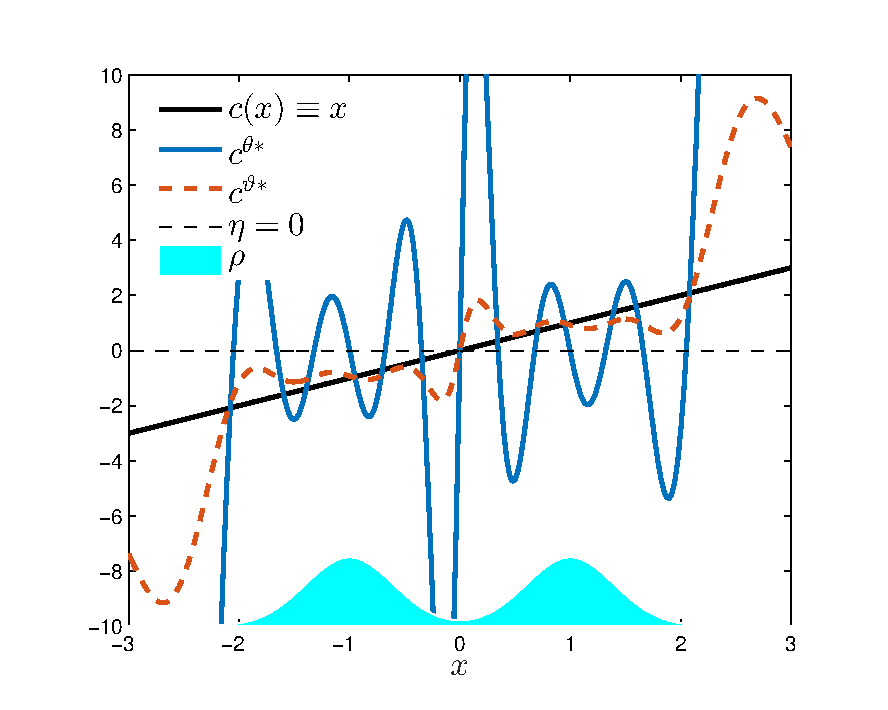
\includegraphics[width=3in]{images/Chap5_x_cvs}} \quad
		\subfigure [] {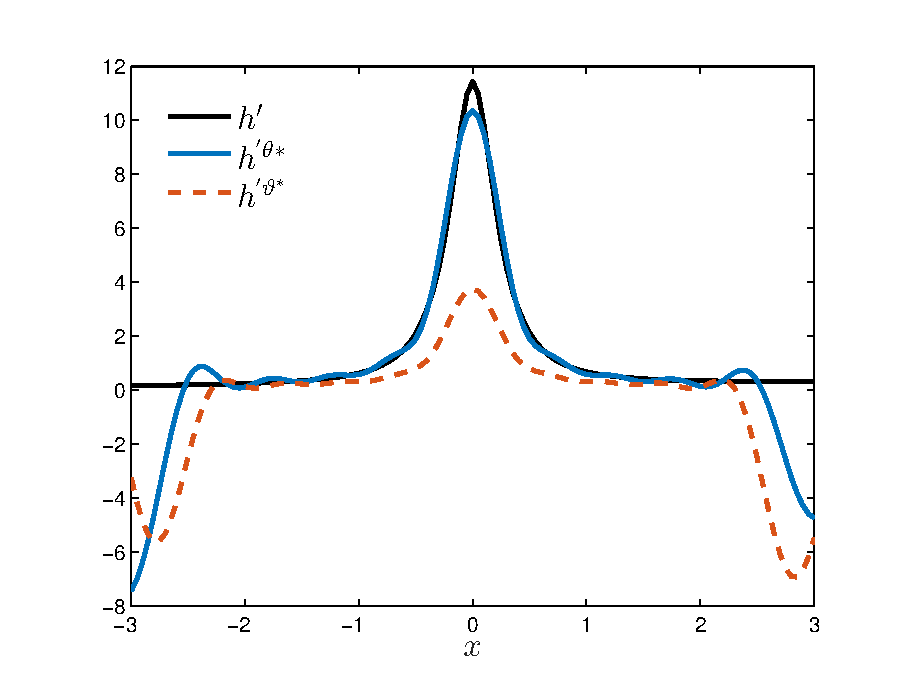
\includegraphics[width=3in]{images/Chap5_x_h_comparison}} 
	}
	\caption{i) Modified estimators using control variates $c^{\theta^*}$ and $c^{\vartheta^*}$, ii) Approximations $h'^{\theta^*}$ and $h'^{\vartheta^*}$ plotted with true gradient $h'$ for $c(x) =x$ with a polynomial $\times \rho_i$ basis.}
	\label{fig:mcmc_cv_theta_var}
\end{figure}


Examining the autocorrelation functions offers another perspective to verify if the two objectives are equivalent. In the discrete time case, the asymptotic variance of the estimates of $\eta$ can be written as the infinite sum of all the autocorrelation functions,
\begin{equation}
\begin{aligned}
\asymvar  & \eqdef \sum_{n=-\infty}^\infty R(n), \qquad R(n) = \Expect [\tilc(\markovstate_0) \tilc(\markovstate_n)] \\
& = 2 \sum_{n=0}^\infty R(n)- R(0).
\end{aligned}
\label{e:mcmc_autocorrelation}
\end{equation}
The expression for $\asymvar$ in \eqref{e:mcmc_avar_reversible} can be derived from this infinite summation form. On inspecting the two objectives, it is easy to see that while $c^{\theta^*}$ tries to minimize $\asymvar$, $c^{\vartheta^*}$ minimizes just the term $R(0)$ in it. This is evident from the the autocorrelation function $R(n)$ in \eqref{e:mcmc_autocorrelation} plotted in \Fig{fig:mcmc_auto_correlation}. Autocorrelation function corresponding to the three different estimators $c,c^{\theta^*}$  and $c^{\vartheta^*}$ for $c(x) = x$, are plotted for $n$ upto $100$. Although, $c^{\vartheta^{*}}$ has the least correlation value at $n=0$ (variance), it shows a slow decay as $n$ increases, $c^{\theta^*}$ shows a much sharper decay in the tails, resulting in a much lower overall asymptotic variance. The plot clearly illustrates that minimizing the variance is not always equivalent to minimizing the asymptotic variance.

\begin{figure}[htbp]
	\centering
	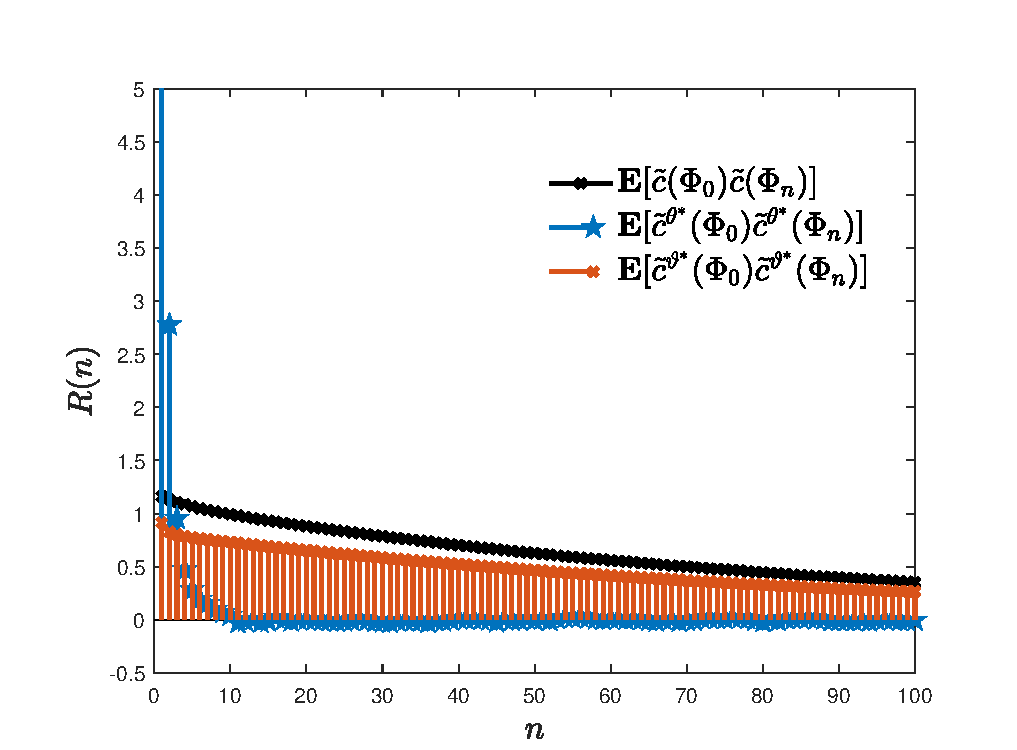
\includegraphics[width=3.5in]{images/Chap5_cov_R_n_gamma_pt05}
	\caption{ Autocorrelation functions $R(n)$ corresponding to the three estimators $c, c^{\theta^*}$ and $c^{\vartheta^*}$  for $n= 0$ to $100$ for ULA with step size $\mcmcstep = 0.05$}
	\label{fig:mcmc_auto_correlation}
\end{figure}

\section{Numerical Examples}
\label{s:mcmc_numerics}
In this section we present a survey of the numerical experiments performed based on the algorithms presented in this paper. We illustrate the remarkable reduction in asymptotic variance that is achieved by the various $\gradTD$ based algorithms, first for estimating the mean of a simple functions $c(x)$ with respect to a univariate Gaussian mixture target density and then in a maximum-likelihood parameter estimation problem using logistic regression.   

\subsection{ULA and RWM for a Univariate Gaussian Mixture Target Density}
\label{s:mcmc_ex_avar}
In this section, we first look at how the control variates are effective in reducing the asymptotic variance for both the ULA and RWM algorithms.  For a simple demonstration of the idea, we consider the same one dimensional bimodal target density defined as mixture of Gaussians \eqref{e:fpf_gaussian_mixture_example}. This gives a symmetric density $\pr$ as shown by the shaded region in \Fig{fig:mcmc_cv_theta_var}. The linear function $c(x) \equiv x$ is used in the simulation experiments; symmetry of $\pr$ and $c$ being an odd function imply $\eta = 0$.

\begin{figure}[htbp]
	\centering
	\mbox{
  	\subfigure[] {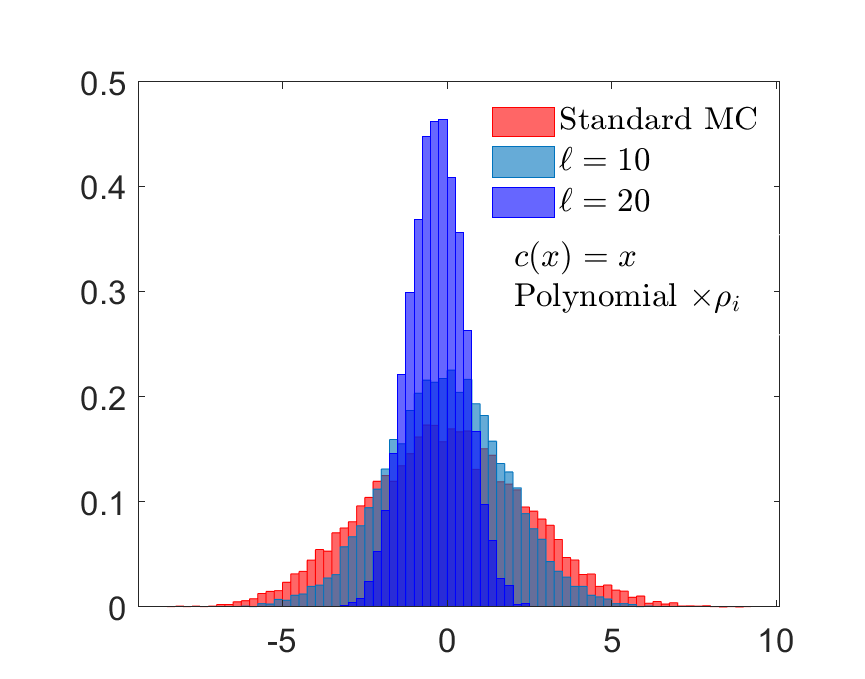
\includegraphics[width=3in]{images/Chap5_hist_all_ds_basis_10000runs_100000samples}}
  	\subfigure[] {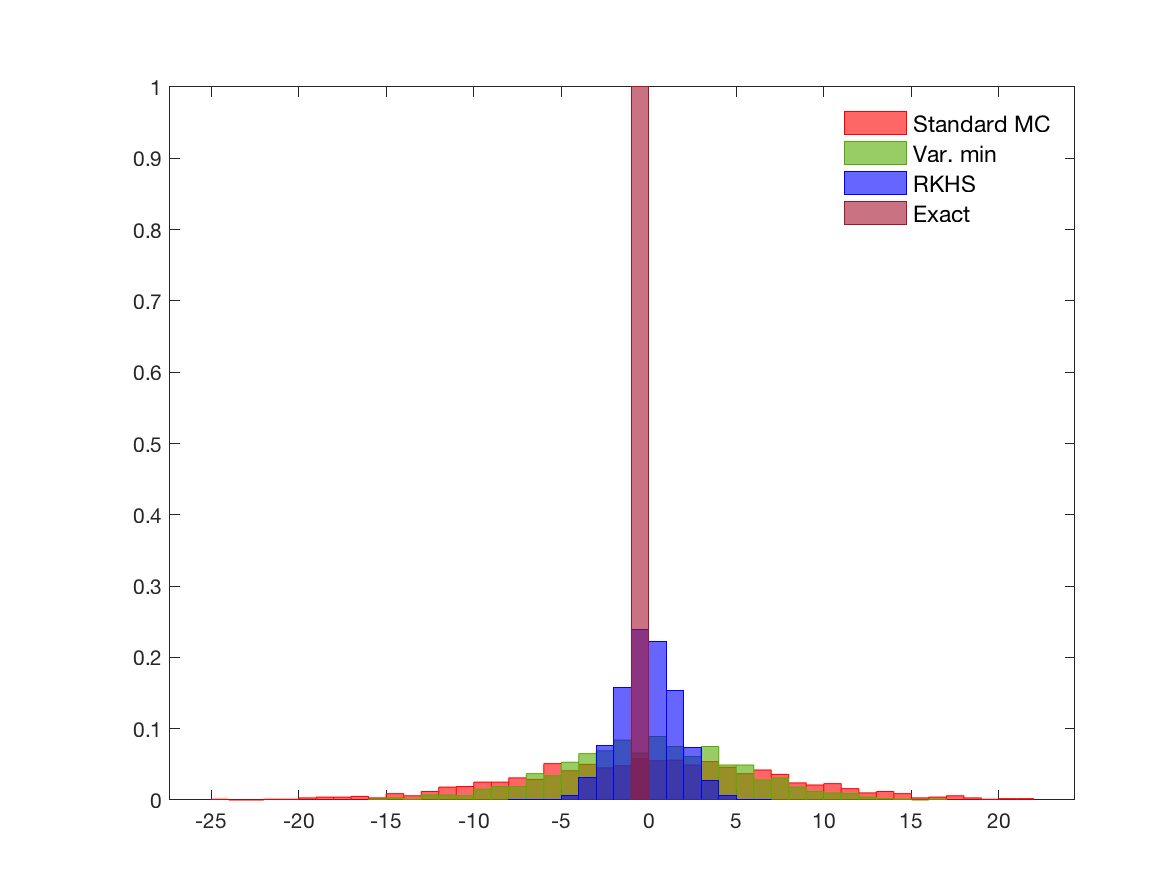
\includegraphics[width=3in]{images/Chap5_hist_asym_var_all_methods}}
  }
 \mbox{
	\subfigure [] {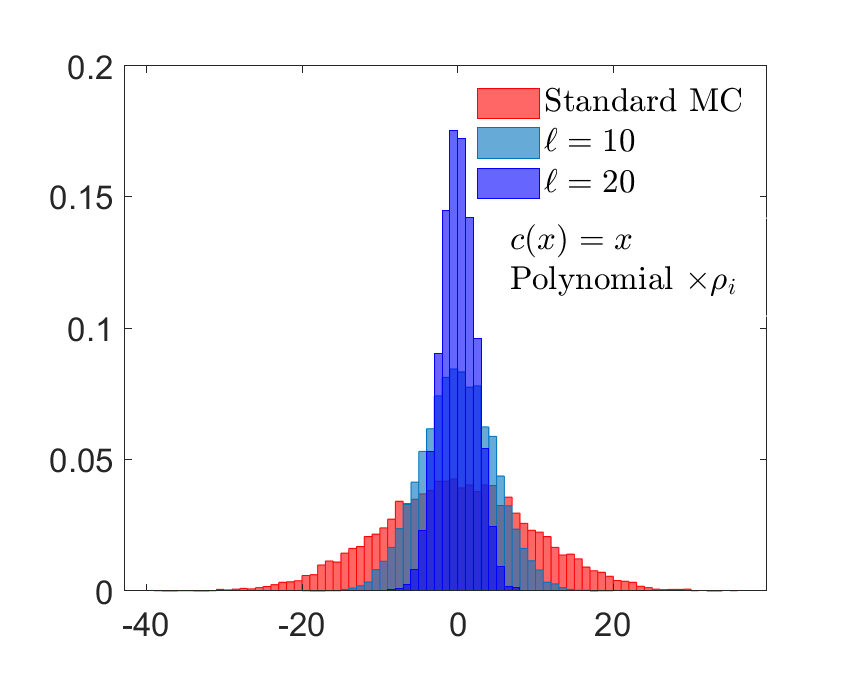
\includegraphics[width = 3in]{images/Chap5_hist_mh_all_ds_basis_10000runs_100000samples}} 
	\subfigure[]	{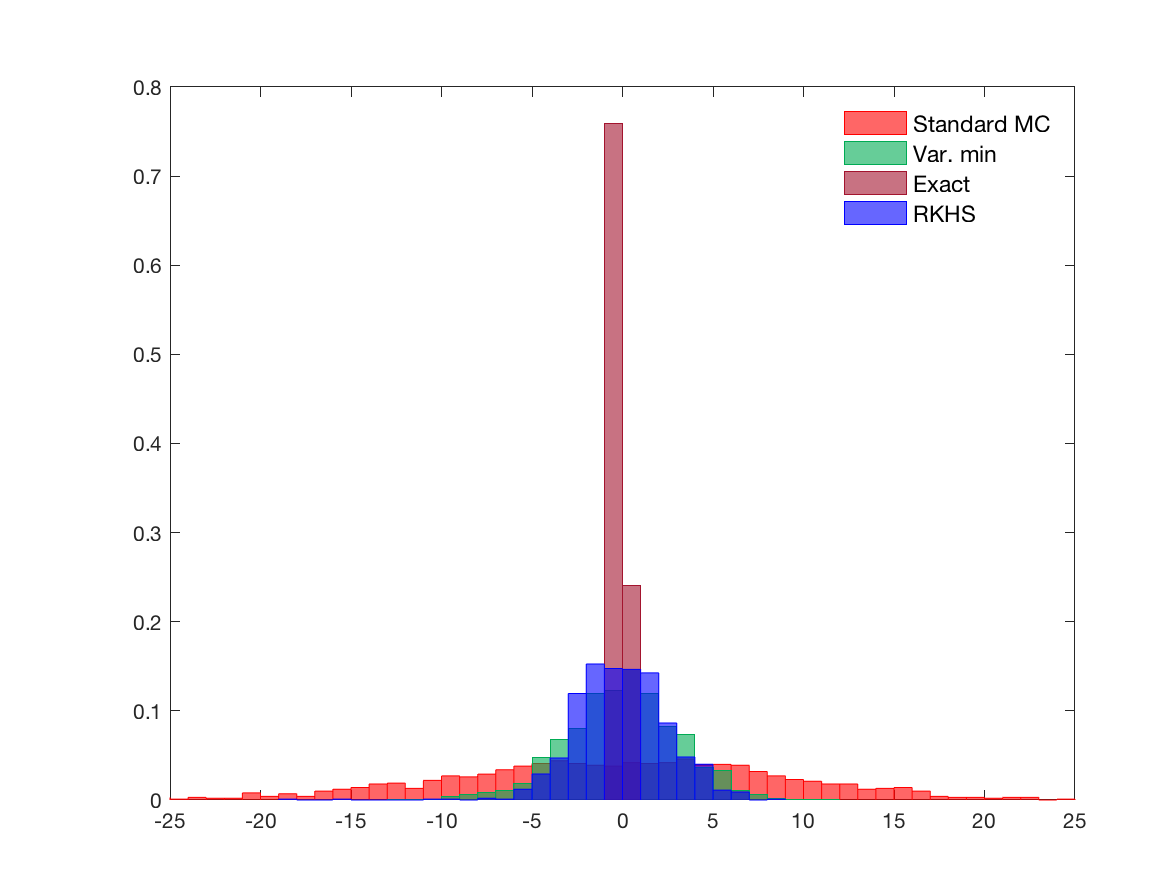
\includegraphics[width=3in]{images/Chap5_hist_mh_asym_var_all_methods}}
 } 
	\caption{Histogram of $\sqrt{N}(\eta_N^{i} - \eta$) for the various control variate schemes -  A) and B) ULA with $\mcmcstep =0.05$ and $c(x) = x$ with finite basis $\ell = 10,20$ in A) and other approximation schemes in B), and C) and D) for RWM with $\mcmcstep = 0.05$ with finite basis $\ell = 10,20$ in C) and other approximation schemes in D).$\ell =0$ corresponds to the standard MCMC estimator.}
	\label{fig:mcmc_ula_rwm_hist}
\end{figure}

Both the ULA and RWM algorithms were simulated using Euler discretization with a step size of $\mcmcstep = 0.05$. Part A in \Fig{fig:mcmc_ula_rwm_hist} shows the histograms of the estimates obtained over $10^4$ independent trials for $\ell= 10,20$ for a weighted polynomial basis, compared to the standard MC estimator. A total number of $10^5$ samples were used in each trial. The empirical variance values observed on the histograms are very close to the analytical variances, although a small bias is seen in the estimate in some cases. This bias may be attributed to the Euler-discretization of the Langevin diffusion which alters the invariant distribution as mentioned in \cite{robtwe96}.  %\Fig{mean_estimate_lang} compares the trajectories of the mean estimate using the standard ULA technique and the improved estimator with the control variates. The improved estimator shows quicker convergence to the actual mean $\eta$ and far fewer fluctuations than the one using the standard technique.

Part B of \Fig{fig:mcmc_ula_rwm_hist} presents a comparison of the performance of the control variates obtained by the other approximation schemes. The histograms were obtained from $1000$ independent trials and the number of samples used in each trial was $N=10^5$. The asymptotic variance obtained by using the exact function $h'$ obtained analytically \eqref{e:fpf_gain_1d} is nearly zero. The $\gradTD$-RKHS algorithm produces the lowest asymptotic variance among approximation methods. Compared to the standard estimator, the variance minimization method (ZV) \cite{papmirgir14} produced nearly the same variance. Markov semigroup approximation method \cite{tagmeh16a} and the constant approximation to $h'$ were also tested, but they produced variances larger than the standard estimator.

The same set of experiments is repeated for the RWM algorithm with the results displayed in parts C and D of \Fig{fig:mcmc_ula_rwm_hist}. Significant reduction in the variance is observed in simulation results. % The intuitive explanation is because of the fact that in the design of $c^\theta$, we try to track $c$ closely using $\generate h^\theta$. Minimizing the error between $h$ and $h^\theta$ tends to minimize the asymptotic variance. In the case of  perfect tracking, $c^\theta$ reduces to the exact mean $\eta$.

\begin{figure}[htbp]
	\centering
		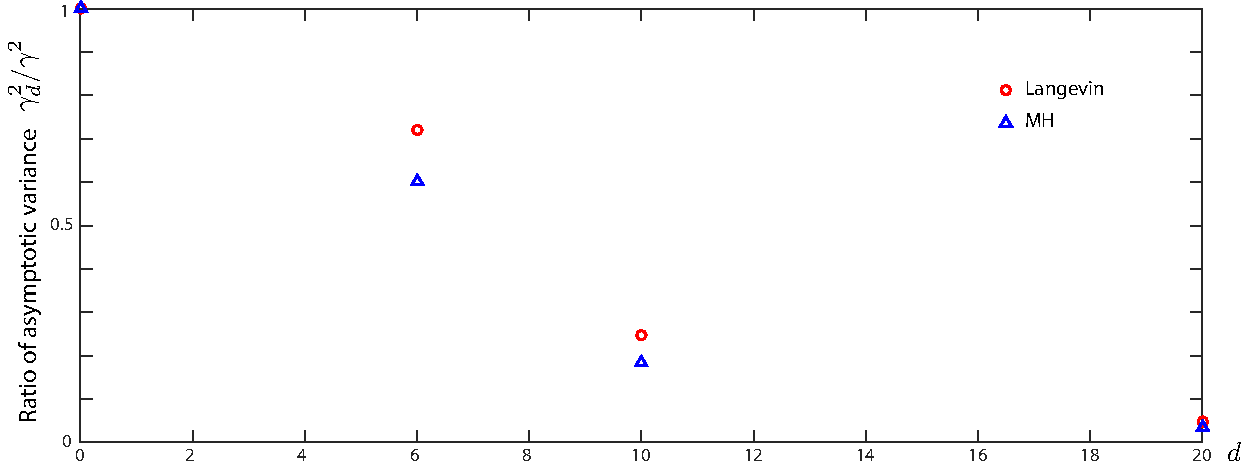
\includegraphics[width=3in]{images/Chap5_rel_red_lang_mh_all}
\caption{Asymptotic variance reduction comparison between ULA and RWM algorithms for $c(x) =x$ and $1\leq \ell \leq 20$}
\label{fig:mcmc_ula_rwm_asy_var}
\end{figure}
\Fig{fig:mcmc_ula_rwm_asy_var} shows the relative reduction in variance for both the ULA and RWM algorithms. The value corresponding to $\ell = 0$ is normalized to $1$ in both the cases. It may be seen that significant variance reduction is achieved for RWM, although at a reduced rate than for ULA. The algorithm can be applied to a wider class of densities with similar results %; we have seen positive results for heavy-tailed densities also. %  Similar trends can also be observed in the Metropolis-Hastings case. \rd{Better results are expected for the Metropolis-Hastings example by applying the algorithm described in \Section{s:cv_reversible_mc}.}

\subsection{Logistic Regression - Swiss Bank Notes Example}
In practice, MCMC algorithms find wide applications in Bayesian inference problems, where we are interested in estimating the mean with respect to a posterior distribution. In this section, we discuss a particular example of Bayesian logistic regression or the logit model. A detailed description of the problem in the context of the Swiss bank notes example is given in \cite{papmirgir14} and a brief summary is provided here.

The goal is to learn the regression coefficients that can be used to classify the Swiss bank notes dataset into genuine and counterfeit. Given in the dataset are the measurements for four covariates - the length of the bill, the width of the left and the right edges and the bottom margin width for 200 bank notes of which 100 each are counterfeit and genuine. This is essentially a binary classification problem in a supervised learning setting. 

Let $X \in \Re^{N_n \times N_d}$ correspond to the covariate measurements of $N_n$ bank notes, with $N_d$ denoting the number of covariates with $N_n = 200$ and $N_d = 4$. Let $\{Y_i  \in \{0,1\}, 1 \leq i \leq N_n \}$ correspond to the labels for each note being genuine or counterfeit respectively. Let $\boldsymbol{\Theta} \in \Re^{N_d}$ be the regression coefficients that are learned from the given data. We are interested in finding the best estimates for the regression coefficients, i.e. the coefficients that maximize the posterior probability $\pr$ defined as,
\begin{equation}
\begin{aligned}
\boldsymbol{\Theta}^* &\eqdef  \argmax_{\Theta \in \Re^{N_d}} \pr(\boldsymbol{\Theta}| \{X_i,Y_i\}_{i=1}^{N_n}) \\
&= \argmax_{\Theta \in \Re^{N_d} }\exp\left( \underbrace{\sum_{i=1}^{N_n} \{Y_i \boldsymbol{\Theta}^\transpose X_i - \log(1+e^{\boldsymbol{\Theta}^\transpose X_i} ) \}}_{\text{Likelihood}} - \underbrace{2^{-1} \boldsymbol{\Theta}^\transpose \Sigma^{-1} \boldsymbol{\Theta}}_{\text{prior}} \right),
\end{aligned}
\label{e:mcmc_log_reg}
\end{equation}
where the parameter vector $\boldsymbol{\Theta} = [ \Theta_1, \dots ,\Theta_{N_d}]$ has a zero-mean Gaussian prior with a covariance matrix $\Sigma$.

In problems such as this, the maximum a posteriori (MAP) estimate is rarely available in closed-form and is hard to compute. Instead, we try to compute the Bayesian estimate: 
\begin{equation}
\boldsymbol{\Theta}_{{bayes}} \eqdef \int_{\Theta \in \Re^{N_d}} \boldsymbol{\Theta} \, \pr(\boldsymbol{\Theta}| \{X_i,Y_i\}_{i=1}^{N_n}) \ud \Theta.
\label{e:mcmc_log_reg_bayes}
\end{equation}
Obtaining the Bayesian estimator \eqref{e:mcmc_log_reg_bayes} requires sampling $\boldsymbol{\Theta}$ values from the posterior distribution and then computing the empirical mean $\hat{\boldsymbol{\Theta}}$. Samples from this posterior density may be obtained using any reversible MCMC technique, in particular we focus on the RWM algorithm. In the following, it is assumed that $N$ samples generated by the RWM algorithm are available.

The goal as before is to compute the optimal control variates that minimize the asymptotic variance of each of the estimates $\hat{\boldsymbol{\Theta}}$.
Optimal control variates can be obtained from approximate solutions to the following Poisson's equations corresponding to each of the four regression coefficients:
\begin{equation}
\generate h_k = -\tilde{\Theta}_k = - (\Theta_k - \hat{\Theta}_k), \qquad   1 \leq k \leq N_d.
\label{e:poisson_logit}
\end{equation}
The approximation $h^\theta_k$ is chosen to belong to a family of linearly parameterized functions as before,
\[
h^\theta_k \eqdef \theta_k^\transpose \psi =  \sum_{j=1}^\ell \theta_{kj} \psi_j,
\]
where $\psi_j : \Re^{N_d} \to \Re$ is the chosen set of basis functions and $\theta_{kj} \in \Re$ are the parameter values.  The optimal parameter values are obtained by minimizing $ \| \nabla h_k - \nabla h^\theta_k \|^2_{L^2}$. For a general basis, the optimal parameter $\theta_k^*$  can be derived along the same lines as before,
\begin{equation}
\begin{aligned}
\theta_k^*  &= M^{-1} b_k, \qquad \text{where,}\\
M & \eqdef \langle \nabla \psi, \nabla \psi \rangle_{L^2} \approx \frac{1}{N} \sum_{i = 0}^{N-1}\nabla \psi(\boldsymbol{\Theta}^i) \nabla \psi^\transpose(\boldsymbol{\Theta}^i)\\
b_k & \eqdef \langle \tilde{\Theta}_k, \psi \rangle_{L^2} \approx \frac{1}{N} \sum_{i=0}^{N-1}\tilde{\Theta}_k^i \psi(\boldsymbol{\Theta}^i), \\
\label{e:theta_k}
\end{aligned}
\end{equation}
where each $\boldsymbol{\Theta^i}$ corresponds to the $i^{\text{th}}$ sample of the MCMC algorithm

Polynomials of degree $1$ and $2$ are chosen as the basis functions in \cite{papmirgir14} and we use the same basis for comparing the algorithm performances. Additionally, we also compare the results against the $\gradTD$-RKHS algorithm with Gaussian kernels. 

\noindent \subsubsection*{Linear polynomial basis}
First we choose $\ell=4$ and $\psi_j$ to be polynomial of degree $1$, i.e.
\begin{equation}
\psi^\transpose \eqdef [ \Theta_1 \quad \Theta_2 \quad \Theta_3 \quad \Theta_4] := \boldsymbol{\Theta}^\transpose
\label{e:mcmc_log_reg_linear}
\end{equation}
For this choice of $\psi$,  $\nabla \psi = I$ and $ \Delta \psi = 0$. Hence, $\theta^*_k$ has the simple expression,
\begin{equation}
\theta^*_k = \frac{1}{N} \sum_{i=0}^{N-1} \tilde{\Theta}_k^i \boldsymbol{\Theta}^i
\label{e:mcmc_log_reg_theta_lin_poly}
\end{equation}
The control variate $\generate h^\theta_k$ is explicitly computable and is given by,
\[
\generate h^\theta_k(\boldsymbol{\Theta}^i) = -\nabla \log(\pr(\boldsymbol{\Theta}^i|\{X_j,Y_j\}_{j=1}^N)) \cdot \theta^*_k \qquad \forall k, i
\]
and the new estimator of the regression coefficients will be,
\[
\bar{\Theta}^i_k \eqdef \Theta^i_k + \generate h^\theta_k(\boldsymbol{\Theta}^i).
\]
The ZV-MCMC algorithm, proposed in \cite{papmirgir14} minimizes the ordinary variance instead of the asymptotic variance. In general, it is an easier optimization problem to solve, but in this specific example, it is interesting to note that $\theta_k^*$  using \eqref{e:mcmc_log_reg_theta_lin_poly} is simpler to compute and the solution is numerically more stable (as inverting an ill-conditioned matrix is not required) than the ZV method. This is denoted as $\gradTD$-L in the plots in \Fig{fig:mcmc_box_plots_Theta}. 

\noindent \subsubsection*{Quadratic basis}
A quadratic polynomial basis of the form,
\begin{equation}
\psi^\transpose \eqdef [\Theta_1, \, \Theta_2, \, \Theta_3, \, \Theta_4, \, \Theta_1^2, \, \Theta_1 \Theta_2, \, \Theta_1\Theta_3, \, \Theta_1 \Theta_4, \, \Theta_2^2, \, \Theta_2\Theta_3, \, \Theta_2\Theta_4, \, \Theta_3^2, \, \Theta_3 \Theta_4, \, \Theta_4^2] 
\label{e:mcmc_log_reg_quadratic}
\end{equation}
is also considered similar to \cite{papmirgir14}.  In this case, $\nabla \psi \in \Re^{14 \times 4}$ and $\theta_k \in \Re^{14}$. The optimal parameter values are given by \eqref{e:theta_k}. This is denoted as $\gradTD$-Q in the plots in \Fig{fig:mcmc_box_plots_Theta}.

\noindent \subsubsection*{$\gradTD$-RKHS algorithm}
We also investigate the performance of the RKHS based $\gradTD$ learning algorithm for this example.  The parameter values of $\lambda = 10^{-7}$ and $\epsy = 2$ were found to produce the best results.  As it becomes prohibitively expensive to place a Gaussian kernel at each of the RWM samples, they were placed at $200$ randomly chosen samples.
\noindent \subsection*{Results}
Simulations were performed using the Swiss bank note dataset provided in \cite{papmirgir14}. We performed $1000$ independent trials each with  $10^5$ samples and $10^4$ samples used for burn-in. The box plots of the estimates of the four regression coefficients $\boldsymbol{\Theta}$ shown in \Fig{fig:mcmc_box_plots_Theta} indicate that significant variance reduction is  achieved using all the control variate methods. It may be observed that for a linear basis, both the ZV-L and $\gradTD$-L learning produce nearly the same asymptotic variance. The $\gradTD$ method is able to produce estimates for the four regression coefficients, whose variance values are $10-65$ times smaller than the standard RWM sampler. Using the quadratic polynomial basis, ZV-Q method outperforms the $\gradTD$-Q method slightly, a variance reduction factor of $100-200$ over the standard estimator is still obtained. The $\gradTD$-RKHS method produces the best results with variances that are lower by a factor $20-50$ over the ZV-Q method. The $\gradTD$-RKHS method however produced a much larger number of outliers. By a more careful choice of the values for $\lambda,\epsy$ and by placing the kernel functions at more well-chosen samples, better results may be obtained.

\begin{figure}[htbp]
	\centering
	\mbox{
		\subfigure [] {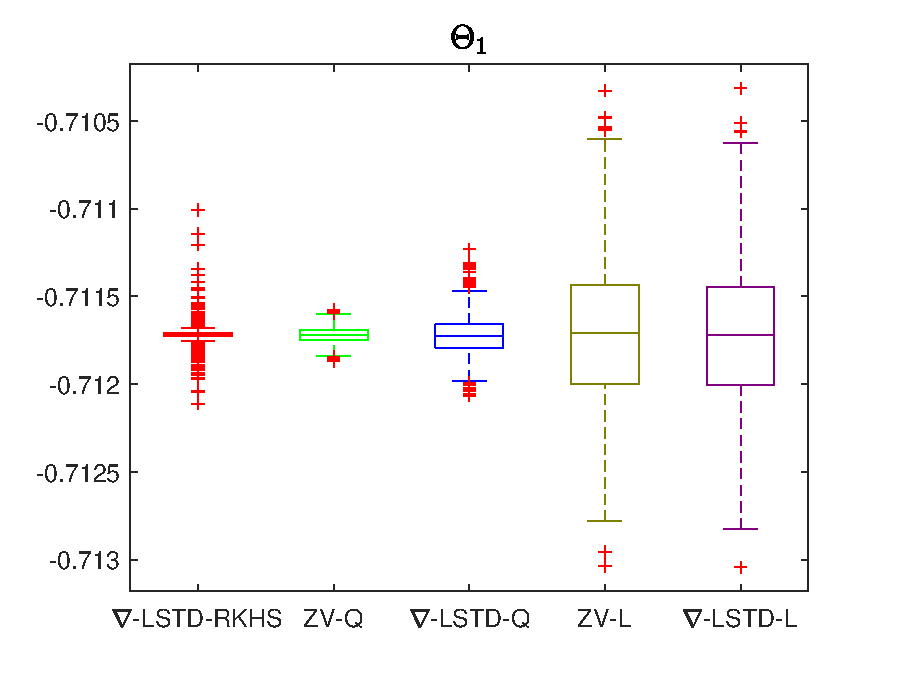
\includegraphics[width=3.5in]{images/Chap5_hist_Theta1_no_std}}
		\subfigure [] {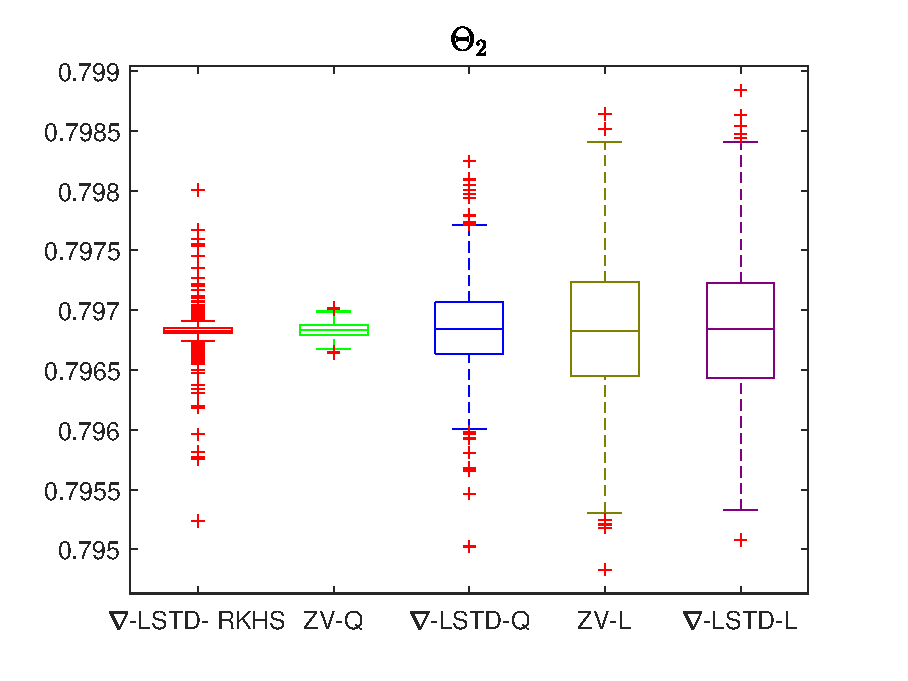
\includegraphics[width=3.5in]{images/Chap5_hist_Theta2_no_std}} 
	}
	\mbox{
		\subfigure [] {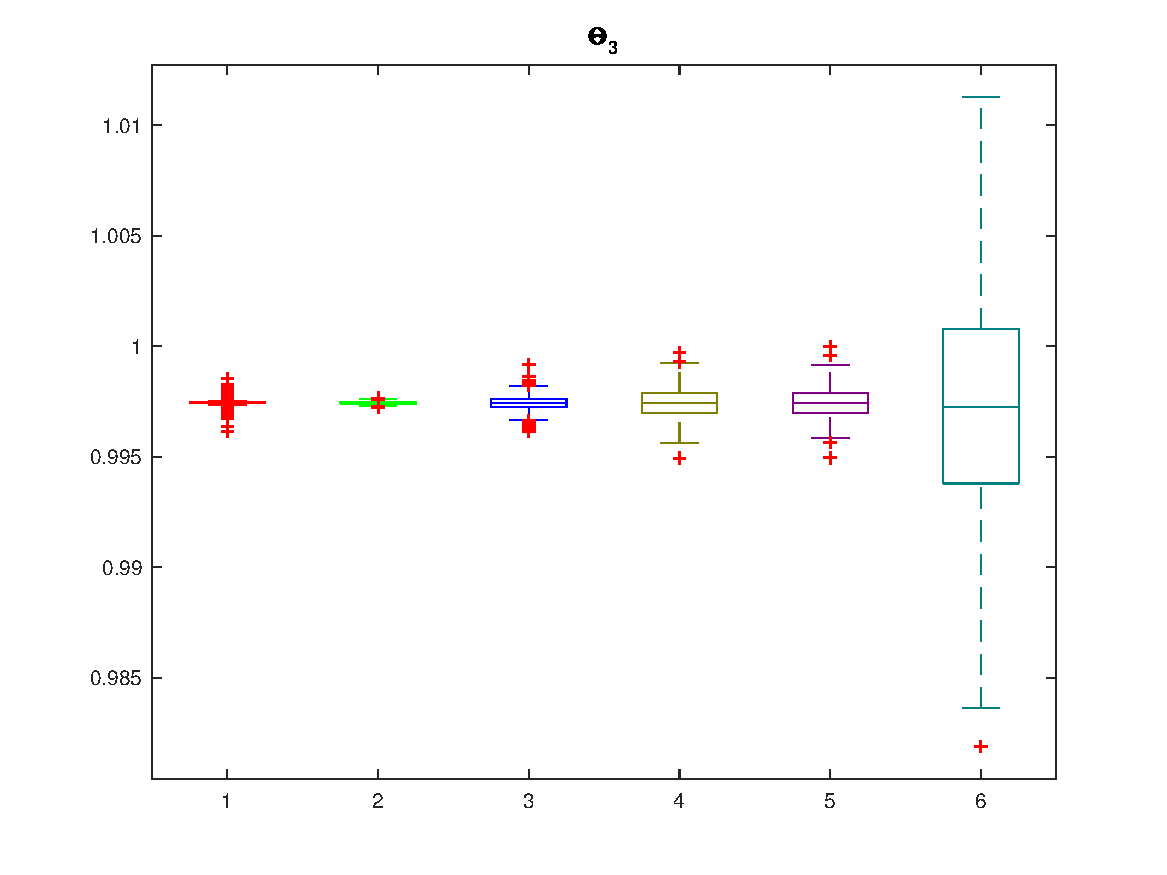
\includegraphics[width = 3.5in]{images/Chap5_hist_Theta3_no_std}} 
		\subfigure [] {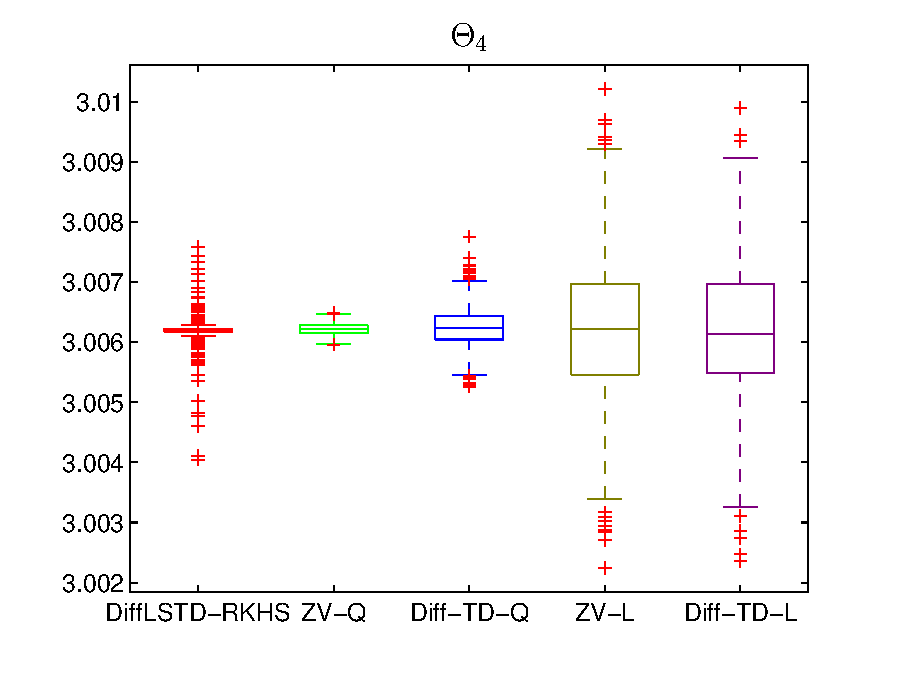
\includegraphics[width = 3.5in]{images/Chap5_hist_Theta4_no_std}} 
	} 
	\caption{Boxplots of estimates of $\boldsymbol{\Theta}$ obtained over 1000 trials using linear and quadratic polynomial basis using the ZV-MCMC and $\gradTD$ and the $\gradTD$-RKHS algorithms).}
  \label{fig:mcmc_box_plots_Theta}
\end{figure}

One might also be interested in the ordinary variance of the samples within a single run. The box plots in \Fig{fig:mcmc_box_var_Theta} compare the variance values of the samples obtained within a run using the ZV-Q method and the $\gradTD$-RKHS learning method. It may be observed that in spite of having outliers, the mean variance using the RKHS method is about one order of magnitude lower than the ZV-Q method.

The same set of experiments were tried out with similar results for the logistic regression example using MALA and ULA sampling. Similar results were also obtained for the probit model Vaso constriction example discussed in \cite{papmirgir14}. The plots for these simulations are provided in the appendix. %\anand{Should I include those plots?}

\begin{figure}[htbp]
	\centering
	\mbox{
		\subfigure [] {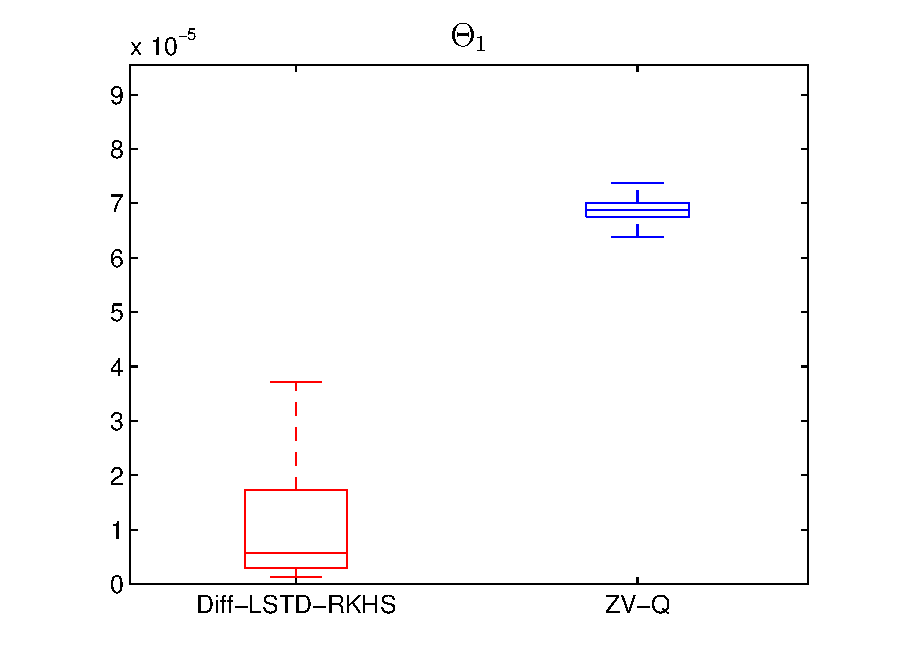
\includegraphics[width=3.5in]{images/Chap5_box_var_Theta1}}
		\subfigure [] {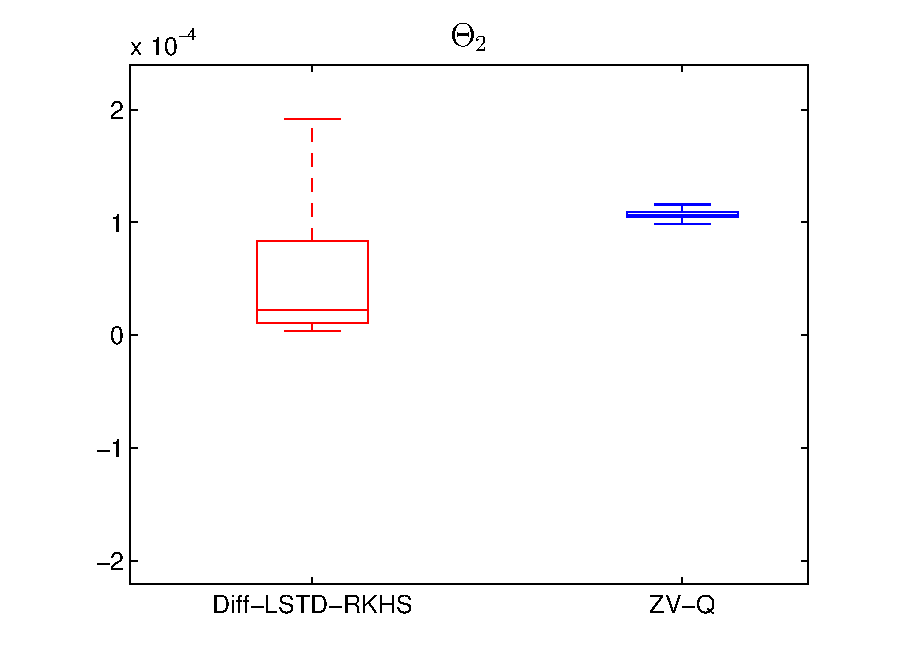
\includegraphics[width=3.5in]{images/Chap5_box_var_Theta2}} 
	}
	\mbox{
		\subfigure [] {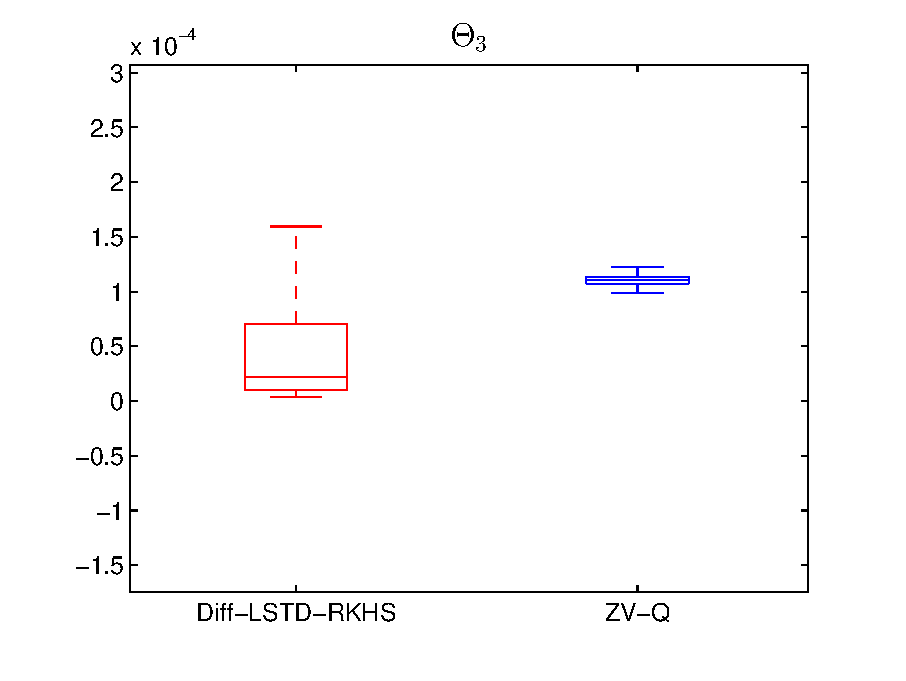
\includegraphics[width = 3.5in]{images/Chap5_box_var_Theta3}} 
		\subfigure [] {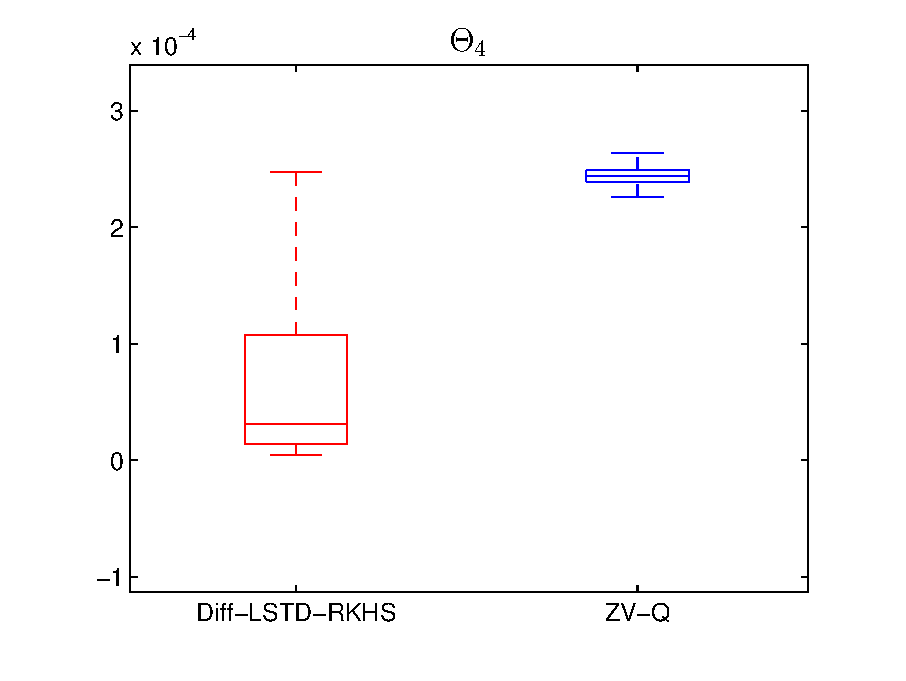
\includegraphics[width = 3.5in]{images/Chap5_box_var_Theta4}} 
	} 
\caption{Boxplots of the in-trial variances of estimates of $\boldsymbol{\Theta}$ obtained over 1000 trials using the $\gradTD$-RKHS and ZV-Q with quadratic polynomials}
\label{fig:mcmc_box_var_Theta}
\end{figure}

\section{Conclusions}
In this chapter, we provided a brief discussion on MCMC algorithms, particularly the ULA, which has an associated continuous time Langevin diffusion process. MCMC algorithms have been widely used in Bayesian inference, as a means of approximating expectations using numerical integration. Asymptotic variance was defined as a measure of convergence of these algorithms. We illustrated using an example that the simpler task of minimizing the variance is not always equivalent to minimizing the asymptotic variance, in fact in certain examples minimizing one quantity produces undesirable results on the other. For the Langevin based algorithms, using \Prop{prop:lang_generator_grad}, we are able to express the asymptotic variance minimization problem in a form that fits into the $\gradTD$ learning objective function. This immediately opens up the application of the various versions of $\gradTD$ learning algorithms discussed in the previous chapters to be applied to this problem. The effectiveness of these techniques is however not limited to ULA, they are also seen to produce significant variance reduction in MALA and RWM algorithms. Through recent research, we have sought theoretical justification for the positive numerical results.  
